\documentclass[11pt,a4paper]{article}
\usepackage[utf8]{inputenc}
\usepackage[francais]{babel}
\usepackage[T1]{fontenc}
\usepackage{amsmath}
\usepackage{amsfonts}
\usepackage{amssymb}
\usepackage{hyperref}
\usepackage{graphicx}
\usepackage{listings}
\usepackage{color}
\usepackage{minted}

% "define" Scala
\lstdefinelanguage{scala}{
  morekeywords={abstract,case,catch,class,def,%
    do,else,extends,false,final,finally,%
    for,if,implicit,import,match,mixin,%
    new,null,object,override,package,%
    private,protected,requires,return,sealed,%
    super,this,throw,trait,true,try,%
    type,val,var,while,with,yield},
  otherkeywords={=>,<-,<\%,<:,>:,\#,@},
  sensitive=true,
  morecomment=[l]{//},
  morecomment=[n]{/*}{*/},
  morestring=[b]",
  morestring=[b]',
  morestring=[b]"""
}

\lstset{language=scala,
	numbers=left,
	frame=single,
	keywordstyle=\color{blue},
	breaklines=true
}

\title{Getting Started}
\author{Nicolas Joseph, Raphaël Gaschignard\\ Guillaume Blondeau, Cyprien Quilici, Jacob Tardieu}

\begin{document}
\maketitle

\section{Overview}
  This document is meant as a "getting started" guide for the \texttt{VivaldiGSI} project, which is an implementation of the Vivaldi algorithm in Scala (hosted on Github at \verb|https://github.com/BeyondTheClouds/VivaldiGSI|). For more specific information on archtecture decisions , check the project's \verb|README|.
  
    This project uses \verb|sbt| as its dependency management and testing system. To generate the intial project files for IntelliJ (our recommended IDE), simply run \verb|sbt gen-idea| in the project root.
    
\section{Architecture}

\begin{figure}[h]
   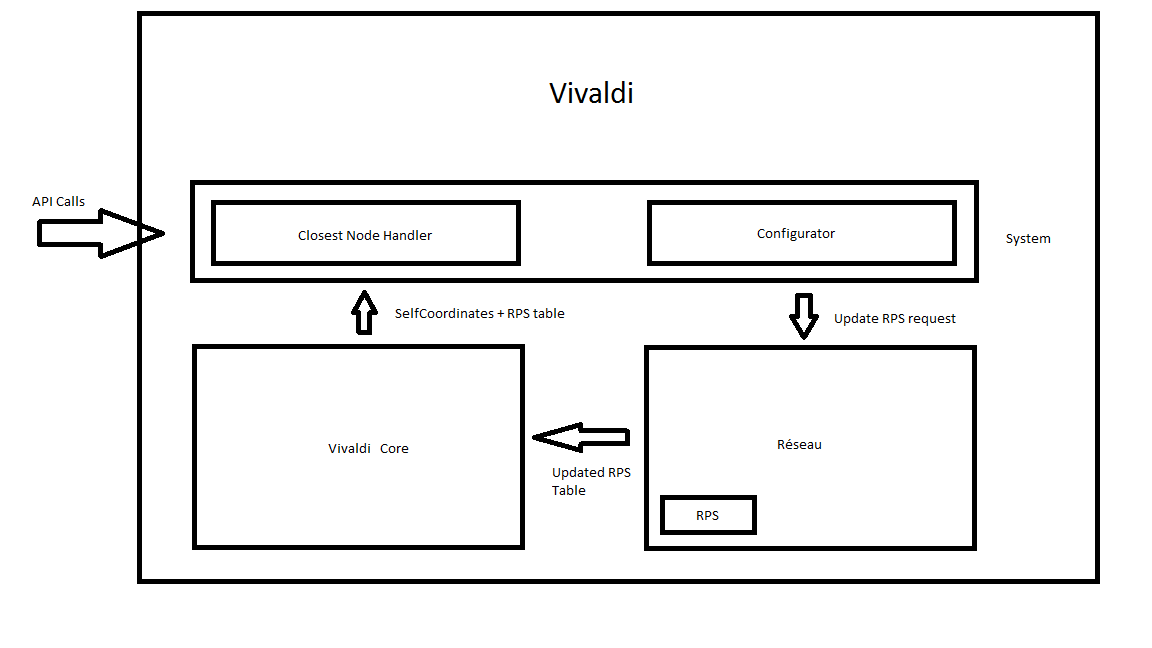
\includegraphics[scale=0.4]{VivaldiArchitecture}
   \caption{\label{acteur} Actor Model}
\end{figure}

The project is built on top of the message-passing actor model, and the API itself (described in the project's \verb|README|) works through message passing (via Akka's \verb|ask| patter) . Here is an overview of the three actors that make our system. 
\begin{itemize}
	\item[$\bullet$] \verb|VivaldiActor| : This actor is the main overlay for our program, and is the one to which API calls should be sent to. This actor sets up the other actors, sets up timers for which to periodically contact other nodes in our network, and update our information. It contains an array of the nodes which are thought to be closest to this actor.
	
	\item[$\bullet$] \verb|Communication| : 
	   This actor maintains a random set of other nodes in our network (called the RPS). This actor , after receiving a signal from the \verb|VivaldiActor|, will contact all the nodes in this set to generate a new random set (by "pinging" the nodes and receiving their RPSs, and current positions). After receiving this information, it is forwarded to the \verb|ComputingAlgorithm| for it to apply the Vivaldi algorithm.
		
	\item[$\bullet$] \verb|ComputingAlgorithm| : This node, after receiving information concerning the position of other nodes in the system, recalculates the current node's position, then sends it to \verb|VivaldiActor| to update its table of the closest nodes in the system.
\end{itemize}


\section{Setting up a network}

 Initializing a node is as simple as creating a new \verb|VivaldiActor|
 \begin{lstlisting}
  val aNode= new VivaldiActor("NodeOne", 1)
 \end{lstlisting}
 
 The node takes a human-readable name and a unique id (used for joining Ping results and used when trying to decide on the equality of actors). 
 
 To connect to an existing network, send the \verb|FirstContact| message to your node, with an \verb|ActorRef| to some other node in your decentralized network.
 
 If you are trying to create a new network, you have two choices : 
 
 \begin{itemize}
    \item Make the node connect to itself 
    \begin{lstlisting}
aNode ! firstContact(aNode.self)
    \end{lstlisting}
 	\item Create the first two nodes and connect them to each other 
 	\begin{lstlisting}
 aNode ! firstContact(anotherNodeRef)
 //in some other program running elsewhere
 anotherNode ! firstContact(aNodeRef)
 	\end{lstlisting}
 \end{itemize}
 
 In any  case, you need to send a \verb|firstContact| message to all nodes, because this is what triggers the schedulers that run all the update code: without this, while nodes can receive information, they will not broadcast their existence in the networks.
 

\section{Defining another distance metric}

By default the metric used for defining distance between two nodes in the overlay is the time it takes for a \verb|Ping| message to make a round-trip on the network. However, sometimes, we want to modify this metric according to other parameters in the system (such as the bandwidth available in a system).

Doing this is relatively easy in our system. One just needs to inherit our \verb|Communications| actor and override the \verb|CalculatePing|  function.

As an example, for our tests running on just one machine, instead of using the round-trip time, we use a predefined map to determine what value to use for each pair of machines (to be able to manually define a topology).

\begin{lstlisting}[language=scala]
class FakePing(id:Long, core:ActorRef, main:ActorRef) extends Communication(id, core, main) {

  /**
   * Gives the ping from the ping table created in the function createTable
   * @param sendTime
   * @param otherInfo
   * @return
   */
   override def calculatePing(sendTime:Long,otherInfo:RPSInfo):Long={

    var ping = FakePing.pingTable(this.id.toInt)(otherInfo.id.toInt)
    ping += Random.nextDouble()/10*Math.pow(-1, Random.nextInt(10))*ping
    ping.toLong
   }
}
\end{lstlisting}

In order to actually run this, we also needed to override our \verb|VivaldiActor| class to use this derived communication class

\begin{lstlisting}[language=scala]
class FakeMain(name : String, id : Long) extends VivaldiActor(name, id) {

  override val vivaldiCore = context.actorOf(Props(classOf[ComputingAlgorithm], self, deltaConf), "VivaldiCore"+id)
  override val network = context.actorOf(Props(classOf[FakePing], id, vivaldiCore, self), "Network"+id)

}
\end{lstlisting}

(All of this can be found in \verb|FakePing.scala|, in our project files)

From there, we can initialize instances of \verb|FakeMain|, and they will use the updated metrics.

A simple way to build this is to do the following: 
\begin{itemize}
\item Build a service that lets you calculate your metric based off of the ids of nodes 
\item Override the \verb|Communication| class with a \verb|calculatePing| that calls this service
\item Override the \verb|VivaldiActor| class to use this updated \verb|Communication| class.
\end{itemize}

\section{Monitoring}
We also built a monitoring application alongside this project. The aim of the monitoring app is to aggregate data from all distributed node to make sure that the system behaves properly. The Monitoring application can be found \href{https://github.com/callicles/VivaldiMonitoringPlay}{Here}.\\

It is very easy too use and deploy. You have a deploy script in the  \texttt{PythonDummyDataGenerator} folder.\\

As far as configuration goes in the Vivaldi part, you need to activate the monitoring in the configuration file and set up the adress of the server the monitoring is being deployed on. You can find all these settings in the \texttt{application.conf} of the Vivaldi project.\\

Here is a proper configuration to use the monitoring :
\begin{minted}[
    frame=single,
  ]{yaml}
# configuration file for the project

akka {

    loggers = ["akka.event.slf4j.Slf4jLogger"]

    # Options: OFF, ERROR, WARNING, INFO, DEBUG
    loglevel = "DEBUG"


}

vivaldi {

    system {

        # Here is the monitoring settings for Vivaldi
        monitoring {
	#Activates the monitoring
            activated = true
	#Url of the monitoring app server
            url = "http://vivaldi-monitoring-demo.herokuapp.com"
	#network name to post data on. You can choose
	#whatever name you would like as long as there is a 
	#corresponding network created in the monitoring app.
            network = "Vivaldi"
        }

        init {

            firstCallTime = 0
            timeBetweenCallsFirst = 1
            timeBetweenCallsThen = 2
            numberOfNodesCalled = 10
            changeTime = 6

        }

        closeNodes {

           size = 100

        }

        vivaldi {

            delta = 0.5

        }

        communication {

            rpssize = 100

        }

    }

}
\end{minted}

As far as the monitoring is concerned, as soon as it is deployed, you just have to create the network you want use. To do so, you can either post a request on the application API or create it manually from the interface. There is a complete API documentation in the README of the GitHub Project. 

\section{Where to go from here}
 Here are a couple things we noted that we would have loved to setup, but didn't have the time to do :
 
 \begin{itemize}
 	\item[$\bullet$]\emph{Create a mechanism to determine configurations }
 	
	A big issue we have currently is that some of the configuration values used for the Vivaldi algorithm are not necessarily optimized for most use cases. Building an automated testing mechanism that could try to find good results (or that could make these parameters vary dynamically) would make the system give better results
	
	\item[$\bullet$] \emph{Use Dependency Injection}
		
	Some aspects of the system(notably the metrics definitions) should be highly configurable, to suit the needs of different users. Currently, the way to do that is through sub-classing, but (as seen in the previous section) that can quickly become unwieldy. Setting up proper dependency injection would solve this.
	
	\item[$\bullet$] \emph{Create better automated testing tools}
	
	We have some tests in place, and we have a monitoring tool to allow for live analysis of a network, but our tools for post-mortem analysis are lacking. While we have logging tools available, some visualization tools for automated post-mortem analysis could be useful.

	\item[$\bullet$] \emph{Monitor Network Usage}
	
	The system works. However, we don't have any experimental data of the network use for our system. It could be useful to know how much bandwidth it needs, could it still be optimized ?  
	 
 \end{itemize}


\end{document}